\chapter{Geografía y teoría económica}

\section{Introdución}

    La agrupación de actividades económicas se puede encontrar en varios niveles de agregación: la variación considerable en el tamaño económico de las ciudades o regiones a nivel nacional, o la distribución desigual de la riqueza y la producción a nivel mundial.\\
    Por supuesto, surge la pregunta de por qué la ubicación parece ser tan importante para las actividades económicas.

\section{La geografía en la economía regional y urbana}
La economía regional y la geografía económica ahora difieren. La economía regional (también conocida como ciencia regional) se basa en la teoría económica neoclásica y es, en efecto, la sucesora formalizada de la tradición alemana de la economía de ubicación. La geografía económica, por otro lado, es más ecléctica y orientada empíricamente. Se inspira en teorías económicas heterodoxas y, cada vez más, en áreas externas a la economía, como la sociología, las ciencias políticas y la teoría de la regulación.\\
Comenzamos con una descripción general de un campo de estudio más joven, a saber, la economía urbana, que estudia la estructura espacial de las áreas urbanas.

\subsection{La economía urbana}
La distribución desigual de la actividad económica dentro de cada país es el punto de partida para la economía urbana. El análisis moderno de la aglomeración de empresas y personas en ciudades o áreas metropolitanas se basa en gran medida en la economía de la aglomeración, un término que se refiere a la disminución de los costos promedio a medida que se produce una mayor producción dentro de un área geográfica específica. En otras palabras se base en rendimientos crecientes a escala. Antes de entrar en la relevancia de las economías de escala para las ciudades y otras formas de aglomeración, primero discutimos un modelo en el que no hay rendimientos crecientes a escala en absoluto. Este modelo, el modelo de ciudad monocéntrica, se origina con von Thu¨nen (1826) y sigue siendo un modelo de referencia para la economía urbana (y regional) hasta el día de hoy. Se justifica una breve discusión, aunque solo sea para poder notar las diferencias con el enfoque de la economía geográfica y dejar claro que, al final, el análisis de las ciudades seguirá siendo bastante limitado mientras no haya rendimientos crecientes a escala.

\subsubsection{El modelo de la ciudad monocéntrica}
El modelo de ciudad monocéntrica asume la existencia de un plano sin rasgos distintivos, perfectamente plano y homogéneo en todos los aspectos. En medio de este plano hay una sola ciudad. Donde existen  agricultores que quieren estar lo más cerca posible de la ciudad para minimizar sus costos de transporte. Este incentivo de estar cerca de la ciudad da como resultado mayores rentas de la tierra cerca de la ciudad que en el borde del plano. Por lo tanto, cada agricultor se enfrenta a una compensación entre las rentas de la tierra y los costos de transporte. Para cada tipo de cultivo existe una curva de oferta-renta que indica, dependiendo de la distancia a la ciudad, cuánto están dispuestos a pagar los agricultores por la tierra.\\
La eficiencia de la asignación de tierras en el modelo monocéntrico depende del supuesto de que no hay externalidades de ubicación.\\
Una serie de hechos estilizados sobre la estructura espacial urbana están de acuerdo con el modelo monocéntrico. Primero, la densidad de población disminuye con la distancia de los centros comerciales centrales. En segundo lugar, casi todas las ciudades importantes del mundo occidental se descentralizaron en el siglo XX (a medida que la gente comenzó a ubicarse más lejos del centro de la ciudad), lo que puede estar relacionado con una caída en los costos de transporte. El modelo monocéntrico también tiene algunas limitaciones serias. Mencionamos solo dos. Primero, el modelo no tiene en cuenta ninguna interacción entre ciudades; no puede ocuparse de los sistemas urbanos. Segundo, el modelo toma la existencia y ubicación de la ciudad como dadas y se enfoca en la ubicación de agricultores/viajeros fuera de la ciudad. \\\\
El término "economías de escala" o "rendimientos crecientes a escala" se refiere a una situación en la que un aumento en el nivel de producción implica una disminución en los costos promedio por unidad de producción para la empresa. Se traduce en una curva de costo promedio con pendiente negativa. Para identificar el origen de la caída de los costes medios, Se distingue entre economías de escala internas y externas. Con las economías de escala internas, la disminución de los costes medios se produce por un aumento del nivel de producción de la propia empresa. Cuanto más produce la empresa, mejor puede beneficiarse de las economías de escala y mayor es su ventaja de costos sobre las empresas más pequeñas. La estructura de mercado que subyace a las economías de escala internas, típicamente utilizada en la literatura de economía geográfica, debe ser necesariamente de competencia imperfecta, ya que las economías de escala internas implican poder de mercado.\\
Con las economías de escala externas, la disminución de los costes medios se produce a través de un aumento de la producción a nivel de la industria en su conjunto, lo que hace que los costes medios por unidad sean una función de la producción de toda la industria. Se distingue aquí entre economías externas puras y pecuniarias. Con economías externas puras (o tecnológicas), un aumento en la producción de toda la industria altera la relación tecnológica entre insumos y producción para cada empresa individual. Por lo tanto, tiene un impacto en la función de producción de la empresa. Un ejemplo de uso frecuente (que se remonta a Alfred Marshall; se refiere a los derrames de información (El derrame de conocimiento ocurre cuando las empresas receptoras explotan el conocimiento que ha sido desarrollado originalmente por una empresa de origen). Estas empresas receptoras pueden ser socios de la alianza, competidores directos de la empresa de origen o empresas de otros sectores industriales). Un aumento en la producción de la industria aumenta el acervo de conocimiento a través de los efectos indirectos positivos de información para cada empresa, lo que lleva a un aumento en la producción a nivel de empresa. En la economía urbana, pero también en la nueva teoría del crecimiento y la nueva teoría del comercio se supone que existen economías externas puras. La estructura del mercado puede entonces ser perfectamente competitiva ya que el tamaño de la empresa individual no importa.\\
Las economías externas pecuniarias son transmitidas por el mercado a través de efectos de precio para la empresa individual, lo que puede alterar su decisión de producción. Dos ejemplos, de nuevo basados en Marshall, son la existencia de un gran mercado local de insumos especializados y la puesta en común del mercado laboral. Una gran industria puede respaldar un mercado de insumos intermedios especializados y un grupo de trabajadores calificados específicos de la industria, lo que beneficia a la empresa individual. A diferencia de las economías externas puras, estos efectos indirectos no afectan la relación tecnológica entre insumos y productos (la función de producción). Las externalidades pecuniarias existen en la literatura de economía geográfica a través de un efecto de amor por la variedad en un gran mercado local. La utilidad de cada consumidor depende positivamente del número de variedades que puede comprar de un bien manufacturado. Los efectos de precio cruciales para las externalidades pecuniarias solo pueden ocurrir con competencia imperfecta. Esto es consistente con el requisito de competencia imperfecta para las economías de escala internas, también utilizado en la literatura de economía geográfica. \\
Algunas observaciones finales están en orden. Primero, los derrames o externalidades son cruciales para las economías externas. El concepto de derrames a veces se utiliza solo para economías externas puras, refiriéndose a las economías externas pecuniarias como un caso de interdependencia del mercado. Nos ceñimos al uso de derrames o externalidades cuando nos referimos a economías de escala externas en general. De manera similar, el término "rendimientos crecientes" a veces se usa solo para economías de escala internas. También usamos la frase “rendimientos crecientes” cuando hablamos de economías externas. Del contexto quedará claro si nos referimos al nivel de la empresa o de la industria. En segundo lugar, las economías externas pueden aplicarse a un nivel de agregación superior al de la empresa. Este suele ser el nivel de la industria, pero en la teoría moderna del comercio y la teoría moderna del crecimiento también puede ser la economía en su conjunto. Tercero, las economías externas en los modelos son estáticas, mientras que la literatura también considera economías externas dinámicas. En ese caso, los costos promedio por unidad de producción son una función negativa de la producción acumulada de la industria. Nuevamente, si esto es relevante, quedará claro si nos referimos a economías externas estáticas o dinámicas. Cuarto, las economías externas discutidas anteriormente son positivas pero también pueden ser negativos, es decir, un aumento en la producción de una empresa conduce a un aumento en los costos por unidad para otras empresas. Finalmente, una observación sobre la terminología un tanto confusa con respecto a las externalidades económicas regionales o efectos indirectos. Es habitual distinguir entre las externalidades Marshall-Arrow-Romer (MAR) y las externalidades de Jacobs. En ambos casos, el énfasis está en los efectos indirectos regionales (específicos de la ubicación), es decir, las empresas deben estar ubicadas lo suficientemente cerca unas de otras para beneficiarse de estas externalidades. Las externalidades SAM se centran en los efectos indirectos específicos del sector y también se conocen como economía de localización. Las externalidades de Jacobs se centran en los efectos indirectos específicos de la ciudad que cruzan los límites entre sectores individuales. Estos también se conocen como economía de la urbanización. Dado que la distinción entre las externalidades MAR y Jacobs como tales no es descriptiva (y por lo tanto no informativa) y la distinción de localización/urbanización puede ser confusa (ya que ambas son específicas de la ubicación), tal vez sea mejor hablar de sector específico y de ciudad.

\begin{center}
    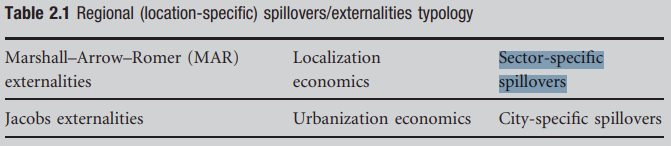
\includegraphics[scale=0.5]{imagen/imagen1.png}
\end{center}

\subsubsection{Economía urbana y rendimientos crecientes}
